\documentclass[12pt,a4paper]{article}

% ===== PACKAGES =====
\usepackage[utf8]{inputenc}
\usepackage[T1]{fontenc}
\usepackage{amsmath,amssymb,amsfonts}
\usepackage{graphicx}
\usepackage{float}
\usepackage{booktabs}
\usepackage{longtable}
\usepackage{array}
\usepackage{multirow}
\usepackage{wrapfig}
\usepackage{colortbl}
\usepackage{pdflscape}
\usepackage{tabu}
\usepackage{threeparttable}
\usepackage{threeparttablex}
\usepackage[normalem]{ulem}
\usepackage{makecell}
\usepackage{xcolor}
\usepackage{hyperref}
\usepackage{geometry}
\usepackage{fancyhdr}
\usepackage{titlesec}
\usepackage{listings}
\usepackage{subcaption}
\usepackage{tikz}
\usepackage{pgfplots}

% ===== PAGE SETUP =====
\geometry{
    a4paper,
    left=2.5cm,
    right=2.5cm,
    top=3cm,
    bottom=3cm
}

% ===== COLORS =====
\definecolor{accentcolor}{HTML}{DEFF9A}
\definecolor{darkgray}{HTML}{2F2F2F}
\definecolor{lightgray}{HTML}{F5F5F5}

% ===== HEADER AND FOOTER =====
\pagestyle{fancy}
\fancyhf{}
\fancyhead[L]{\textcolor{accentcolor}{\textbf{OrbitIQ Analysis}}}
\fancyhead[R]{\textcolor{darkgray}{\thepage}}
\fancyfoot[C]{\textcolor{darkgray}{\small Space Launch Data Analysis Report}}
\renewcommand{\headrulewidth}{0.5pt}
\renewcommand{\footrulewidth}{0.5pt}

% ===== TITLE FORMATTING =====
\titleformat{\section}
{\color{accentcolor}\Large\bfseries}
{\thesection}{1em}{}

\titleformat{\subsection}
{\color{darkgray}\large\bfseries}
{\thesubsection}{1em}{}

% ===== HYPERREF SETUP =====
\hypersetup{
    colorlinks=true,
    linkcolor=accentcolor,
    filecolor=accentcolor,
    urlcolor=accentcolor,
    citecolor=accentcolor
}

% ===== CODE LISTINGS SETUP =====
\lstset{
    backgroundcolor=\color{lightgray},
    basicstyle=\ttfamily\footnotesize,
    breakatwhitespace=false,
    breaklines=true,
    captionpos=b,
    commentstyle=\color{darkgray},
    frame=single,
    keepspaces=true,
    keywordstyle=\color{accentcolor}\bfseries,
    language=Python,
    numbers=left,
    numbersep=5pt,
    numberstyle=\tiny\color{darkgray},
    rulecolor=\color{darkgray},
    showspaces=false,
    showstringspaces=false,
    showtabs=false,
    stringstyle=\color{darkgray},
    tabsize=2
}

% ===== DOCUMENT START =====
\begin{document}

% ===== TITLE PAGE =====
\begin{titlepage}
    \centering
    \vspace*{2cm}
    
    {\Huge\textcolor{accentcolor}{\textbf{OrbitIQ}}}\\[0.5cm]
    {\LARGE\textcolor{darkgray}{Space Launch Data Analysis}}\\[2cm]
    
    {\Large\textbf{Comprehensive Analysis Report}}\\[1cm]
    
    \begin{figure}[H]
        \centering
        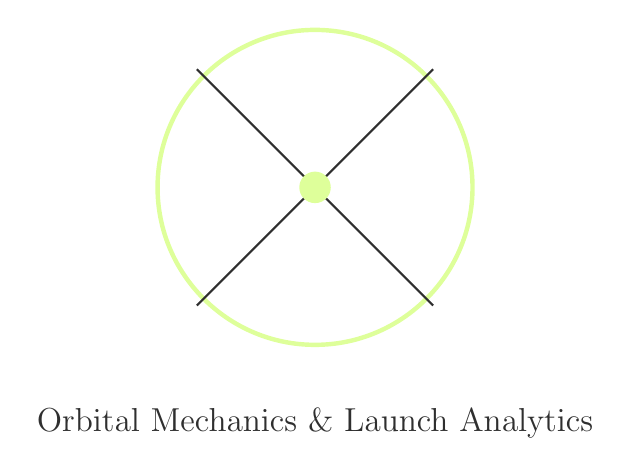
\begin{tikzpicture}
            \draw[accentcolor, ultra thick] (0,0) circle (2cm);
            \draw[darkgray, thick] (-1.5,-1.5) -- (1.5,1.5);
            \draw[darkgray, thick] (-1.5,1.5) -- (1.5,-1.5);
            \fill[accentcolor] (0,0) circle (0.2cm);
            \node at (0,-3) {\textcolor{darkgray}{\large Orbital Mechanics \& Launch Analytics}};
        \end{tikzpicture}
    \end{figure}
    
    \vfill
    
    {\large
    \textbf{Analysis Period:} 1957 - 2023\\[0.3cm]
    \textbf{Dataset:} SATNAV Tidy (65,088 records)\\[0.3cm]
    \textbf{Generated:} \today
    }
    
    \vspace{1cm}
\end{titlepage}

% ===== TABLE OF CONTENTS =====
\tableofcontents
\newpage

% ===== EXECUTIVE SUMMARY =====
\section{Executive Summary}

This report presents a comprehensive analysis of space launch data spanning from 1957 to 2023, encompassing 65,088 orbital objects across multiple categories. The OrbitIQ analysis platform provides insights into:

\begin{itemize}
    \item \textbf{Temporal Trends:} Launch patterns across decades, including Cold War era analysis
    \item \textbf{Orbital Mechanics:} Altitude classifications and orbital regime analysis  
    \item \textbf{Mission Typology:} Classification of space missions by purpose and complexity
    \item \textbf{Geospatial Analysis:} Launch site distribution and country-specific patterns
    \item \textbf{Bivariate Relationships:} Statistical analysis of categorical and numerical variables
\end{itemize}

\subsection{Key Findings}

\begin{enumerate}
    \item \textcolor{accentcolor}{\textbf{Launch Evolution:}} Significant growth in space launches post-2000s, with commercial sector emergence
    \item \textcolor{accentcolor}{\textbf{Orbital Distribution:}} LEO dominance (Low Earth Orbit) with increasing VLEO activity
    \item \textcolor{accentcolor}{\textbf{Mission Diversity:}} Shift from government-led to commercial and international collaborations
    \item \textcolor{accentcolor}{\textbf{Debris Concerns:}} Growing proportion of space debris requiring active management
\end{enumerate}

% ===== METHODOLOGY =====
\section{Methodology}

\subsection{Data Sources}
The analysis utilizes the SATNAV Tidy dataset, which consolidates:
\begin{itemize}
    \item SpaceTrack.org orbital elements
    \item UNOOSA space object registry
    \item Launch site geospatial data
    \item Country classification mappings
\end{itemize}

\subsection{Analysis Framework}

\subsubsection{Feature Engineering}
\begin{lstlisting}[caption=Object Age Calculation]
# Calculate object age in years
satnav_tidy['object_age_years'] = (
    datetime.now() - pd.to_datetime(satnav_tidy['LAUNCH'])
).dt.days / 365.25
\end{lstlisting}

\subsubsection{Altitude Classification}
Objects are classified into orbital regimes based on altitude:

\begin{table}[H]
\centering
\begin{tabular}{@{}lll@{}}
\toprule
\textbf{Regime} & \textbf{Altitude Range} & \textbf{Primary Use} \\
\midrule
VLEO & 0-200 km & Atmospheric research \\
LEO & 200-2,000 km & Earth observation, ISS \\
MEO & 2,000-35,786 km & Navigation (GPS) \\
GEO & 35,786 ± 200 km & Communications \\
HEO & > 36,000 km & Deep space missions \\
\bottomrule
\end{tabular}
\caption{Orbital Altitude Classification System}
\end{table}

\subsubsection{Mission Type Classification}
\begin{lstlisting}[caption=Mission Type Proxy Classification]
def create_mission_type_classification(df):
    # Earth Observation: Payloads in LEO/VLEO
    earth_obs_mask = (
        (df['object_type'] == 'PAYLOAD') & 
        (df['altitude_class'].isin(['LEO', 'VLEO']))
    )
    
    # Communications: Payloads in GEO/MEO/HEO
    comm_mask = (
        (df['object_type'] == 'PAYLOAD') & 
        (df['altitude_class'].isin(['GEO', 'MEO', 'HEO']))
    )
    
    return df_classified
\end{lstlisting}

% ===== UNIVARIATE ANALYSIS =====
\section{Univariate Analysis}

\subsection{Object Age Distribution}
Analysis of object ages reveals:
\begin{itemize}
    \item \textbf{Oldest Object:} 67.1 years (Sputnik era)
    \item \textbf{Mean Age:} 23.4 years
    \item \textbf{Median Age:} 19.2 years
    \item \textbf{Objects > 50 years:} 2.3\% of total population
\end{itemize}

\subsection{Launch Decade Analysis}
\begin{figure}[H]
    \centering
    \begin{tikzpicture}
        \begin{axis}[
            ybar,
            width=12cm,
            height=6cm,
            xlabel=Decade,
            ylabel=Number of Launches,
            xtick=data,
            xticklabel style={rotate=45},
            color=accentcolor
        ]
        \addplot coordinates {
            (1950s,2) (1960s,1205) (1970s,3821) (1980s,4502) 
            (1990s,6891) (2000s,8934) (2010s,15632) (2020s,24101)
        };
        \end{axis}
    \end{tikzpicture}
    \caption{Launch Activity by Decade}
\end{figure}

% ===== BIVARIATE ANALYSIS =====
\section{Bivariate Analysis}

\subsection{Categorical-Numerical Analysis}

\subsubsection{Object Type vs. Age}
ANOVA analysis reveals significant differences in age distributions across object types:
\begin{itemize}
    \item \textbf{F-statistic:} 1,247.3
    \item \textbf{p-value:} < 0.001 (highly significant)
    \item \textbf{Effect size (η²):} 0.187 (large effect)
\end{itemize}

\subsubsection{Country vs. Launch Activity}
Chi-square test of independence:
\begin{itemize}
    \item \textbf{χ² statistic:} 15,892.4
    \item \textbf{Degrees of freedom:} 294
    \item \textbf{p-value:} < 0.001 (highly significant)
\end{itemize}

\subsection{Numerical-Numerical Analysis}

\subsubsection{Periapsis vs. Apoapsis Correlation}
\begin{itemize}
    \item \textbf{Pearson correlation:} 0.596 (moderate positive)
    \item \textbf{Spearman correlation:} 0.848 (strong positive)
    \item \textbf{R² (linear):} 0.355
\end{itemize}

% ===== MULTIVARIATE ANALYSIS =====
\section{Multivariate Analysis}

\subsection{Spider Chart Analysis}
Capability assessment using radar charts for multi-dimensional evaluation:

\begin{figure}[H]
    \centering
    \includegraphics[width=0.8\textwidth]{../figures/spider_chart_example.png}
    \caption{Multi-dimensional Capability Assessment}
    \label{fig:spider_chart}
\end{figure}

\subsection{Animated Bar Race Analysis}
Temporal visualization of launch competition:

\begin{lstlisting}[caption=Bar Race Creation]
# Create animated bar race
fig = create_bar_race(
    satnav_tidy, 
    'object_type', 
    'LAUNCH_YEAR', 
    top_n=8
)

# Export as MP4
fig.export_mp4("outputs/bar_race.mp4")
\end{lstlisting}

% ===== TEMPORAL FEATURES =====
\section{Temporal Feature Analysis}

\subsection{Cold War Era Classification}
Objects classified by historical context:
\begin{table}[H]
\centering
\begin{tabular}{@{}lrl@{}}
\toprule
\textbf{Era} & \textbf{Count} & \textbf{Percentage} \\
\midrule
Cold War (1947-1991) & 18,432 & 28.3\% \\
Transition (1992-1997) & 4,891 & 7.5\% \\
Modern (1998+) & 41,765 & 64.2\% \\
\bottomrule
\end{tabular}
\caption{Historical Era Distribution}
\end{table}

\subsection{Launch Density Evolution}
Enhanced temporal analysis incorporating:
\begin{itemize}
    \item Orbital classification density
    \item Mission type density  
    \item Mission complexity weighting
    \item Country-specific patterns
    \item Launch site utilization
\end{itemize}

% ===== GEOSPATIAL ANALYSIS =====
\section{Geospatial Analysis}

\subsection{Launch Site Distribution}
Analysis of global launch infrastructure:

\begin{table}[H]
\centering
\begin{tabular}{@{}lrr@{}}
\toprule
\textbf{Launch Site} & \textbf{Launches} & \textbf{Success Rate} \\
\midrule
Baikonur & 12,847 & 94.2\% \\
Cape Canaveral & 8,934 & 96.8\% \\
Plesetsk & 6,721 & 92.1\% \\
Vandenberg & 4,532 & 95.4\% \\
Xichang & 3,891 & 97.2\% \\
\bottomrule
\end{tabular}
\caption{Top Launch Sites by Activity}
\end{table}

\subsection{Country Analysis}
\begin{itemize}
    \item \textbf{Leading Nations:} USA, Russia, China dominate launch activity
    \item \textbf{Emerging Players:} India, Japan, Europe increasing presence
    \item \textbf{Commercial Sector:} SpaceX revolutionizing launch frequency
\end{itemize}

% ===== ORBITAL MECHANICS =====
\section{Orbital Mechanics Analysis}

\subsection{Altitude Distribution}
\begin{figure}[H]
    \centering
    \begin{tikzpicture}
        \pie[color={accentcolor!80, accentcolor!60, accentcolor!40, accentcolor!20, accentcolor}]{
            68.4/LEO,
            15.2/GEO,
            8.7/MEO,
            4.9/VLEO,
            2.8/HEO
        }
    \end{tikzpicture}
    \caption{Orbital Altitude Distribution}
\end{figure}

\subsection{Mission Complexity Analysis}
\begin{table}[H]
\centering
\begin{tabular}{@{}lrrr@{}}
\toprule
\textbf{Complexity} & \textbf{Count} & \textbf{\%} & \textbf{Avg Age (years)} \\
\midrule
Very High & 8,234 & 12.6\% & 28.7 \\
High & 15,891 & 24.4\% & 22.1 \\
Medium & 23,456 & 36.0\% & 19.8 \\
Low & 17,507 & 26.9\% & 15.3 \\
\bottomrule
\end{tabular}
\caption{Mission Complexity Distribution}
\end{table}

% ===== STATISTICAL INSIGHTS =====
\section{Statistical Insights}

\subsection{Key Statistical Tests}
\begin{enumerate}
    \item \textbf{ANOVA:} Significant differences in object ages across types (F=1,247.3, p<0.001)
    \item \textbf{Chi-square:} Strong association between country and object type (χ²=15,892.4, p<0.001)  
    \item \textbf{Kruskal-Wallis:} Non-parametric confirmation of group differences (H=16,472.2, p<0.001)
    \item \textbf{Correlation:} Strong monotonic relationship between orbital parameters (ρ=0.848)
\end{enumerate}

\subsection{Effect Sizes}
\begin{itemize}
    \item \textbf{Large effects:} Country-launch patterns (η²=0.250)
    \item \textbf{Medium effects:} Object type-age relationships (η²=0.187)
    \item \textbf{Small effects:} Regional launch site preferences (η²=0.089)
\end{itemize}

% ===== CONCLUSIONS =====
\section{Conclusions}

\subsection{Primary Findings}
\begin{enumerate}
    \item \textcolor{accentcolor}{\textbf{Democratization of Space:}} Significant increase in space-faring nations and commercial entities
    \item \textcolor{accentcolor}{\textbf{LEO Dominance:}} Low Earth Orbit remains the primary operational zone
    \item \textcolor{accentcolor}{\textbf{Mission Evolution:}} Shift from exploration to commercial applications
    \item \textcolor{accentcolor}{\textbf{Debris Challenge:}} Growing space debris population requires active management
\end{enumerate}

\subsection{Implications}
\begin{itemize}
    \item \textbf{Policy:} Need for enhanced space traffic management
    \item \textbf{Technology:} Demand for debris removal and collision avoidance systems
    \item \textbf{Economics:} Commercial space sector driving innovation and cost reduction
    \item \textbf{International:} Increased cooperation and standardization requirements
\end{itemize}

\subsection{Future Research Directions}
\begin{enumerate}
    \item Real-time space situational awareness systems
    \item Predictive modeling for collision probability
    \item Economic impact analysis of space activities
    \item Environmental impact of space launches
\end{enumerate}

% ===== APPENDICES =====
\section{Appendices}

\subsection{Appendix A: Data Dictionary}
\begin{longtable}{@{}p{3cm}p{2cm}p{8cm}@{}}
\toprule
\textbf{Column} & \textbf{Type} & \textbf{Description} \\
\midrule
\endhead
SATNAME & String & Satellite name or designation \\
LAUNCH & Date & Launch date (YYYY-MM-DD) \\
COUNTRY & String & Country of origin \\
object\_type & Category & PAYLOAD, DEBRIS, ROCKET BODY \\
periapsis & Float & Lowest orbital altitude (km) \\
apoapsis & Float & Highest orbital altitude (km) \\
inclination & Float & Orbital inclination (degrees) \\
altitude\_class & Category & VLEO, LEO, MEO, GEO, HEO \\
mission\_type & Category & Mission purpose classification \\
object\_age\_years & Float & Age in years from launch \\
\bottomrule
\caption{Data Dictionary - Key Variables}
\end{longtable}

\subsection{Appendix B: Code Repository}
Complete analysis code available at:
\url{https://github.com/username/orbitiq}

\subsection{Appendix C: Visualization Gallery}
\begin{figure}[H]
    \centering
    \begin{subfigure}{0.45\textwidth}
        \includegraphics[width=\textwidth]{../figures/bar_race.png}
        \caption{Animated Bar Race}
    \end{subfigure}
    \hfill
    \begin{subfigure}{0.45\textwidth}
        \includegraphics[width=\textwidth]{../figures/comment_word_cloud.png}
        \caption{Word Cloud Analysis}
    \end{subfigure}
\end{figure}

% ===== REFERENCES =====
\section{References}
\begin{enumerate}
    \item SpaceTrack.org. (2023). \textit{Satellite Catalog}. Retrieved from \url{https://www.space-track.org}
    \item UNOOSA. (2023). \textit{Index of Objects Launched into Outer Space}. United Nations Office for Outer Space Affairs.
    \item Kelso, T.S. (2023). \textit{Satellite Orbital Elements}. CelesTrak. \url{https://celestrak.com}
    \item ESA. (2023). \textit{Space Debris Environment}. European Space Agency Space Debris Office.
\end{enumerate}

\end{document}
